\section{Vista de Procesos}
A continuación se muestran los diagramas de secuencia diseñados para la interacción entre el usuario ('administrador' y 'empleado') y el sistema de información. 

%Contenido de la vista de procesos
\subsection{Vista de Procesos Empleado} \label{subsec: Vista Procesos Empleado}
\subsubsection{Iniciar Sesión}
En la figura \ref{fig:Diagrama de Secuencia - Iniciar Sesión} se muestra el diagrama de secuencia que corresponde al inicio de sesión y consta de tres partes principales: Mecánico (usuario), Sistema y Base de Datos. El objetivo es poder ingresar al sistema para poder utilizar el sistema y llevar a cabo las diversas tareas implementadas en dicho sistema. Dentro de este diagrama, existen dos opciones:
\begin{itemize}
	\item \textbf{El usuario si existe en la Base de Datos:} Hay al menos un usuario registrado con un nombre de usuario y una contraseña, posteriormente se permite el acceso al sistema con dichas credenciales.
	\item \textbf{El usuario NO existe en la Base de Datos:} No hay ningún registro de algún usuario en la base de datos, el sistema niega el acceso con esas credenciales. Cabe señalar que existe la posibilidad que el usuario ingrese de manera errónea dichas credenciales.
\end{itemize} 
\begin{figure}[!h]
	\centering
	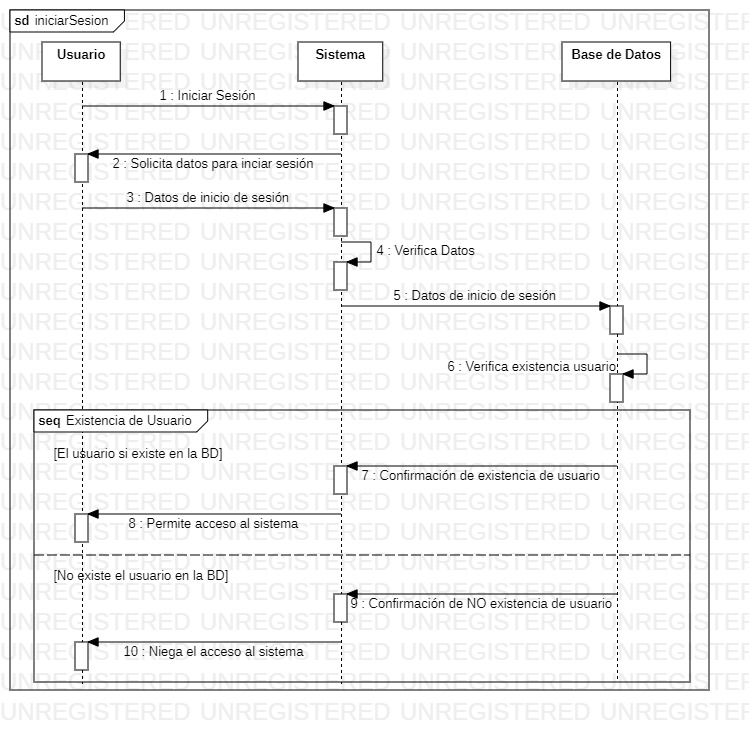
\includegraphics[width=1\textwidth]{./diseno/vprocesos/imagenes/iniciarSesion}
	\caption{Diagrama de Secuencia - Iniciar Sesión}
	\label{fig:Diagrama de Secuencia - Iniciar Sesión}
\end{figure}
\clearpage
\subsection{Visualizar Menú}
En la figura \ref{fig:Diagrama de Secuencia - Visualizar Menú} mostramos el diagrama de secuencia correspondiente a la función de visualizar menú, aquí el Mecánico (usuario) puede elegir dos opciones:
\begin{itemize}
	\item \textbf{Gestión de Agenda:} Al elegir esta opción, el usuario podrá entrar a otra parte del sistema para que pueda interactuar con la base de datos mediante una interfaz gráfica. Es decir, que llevará a cabo las diversas tareas para poder tener un control sobre la información a cerca de los vehículos a reparar.
	\item \textbf{Gestión de Refacciones:} Si el usuario elige esta opción, el usuario podrá visualizar las refacciones que existen en el almacén del taller. En caso de que no exista la pieza que el necesita, podrá generar una solicitud dentro del mismo sistema. 
\end{itemize}
\begin{figure}[!h]
	\centering
	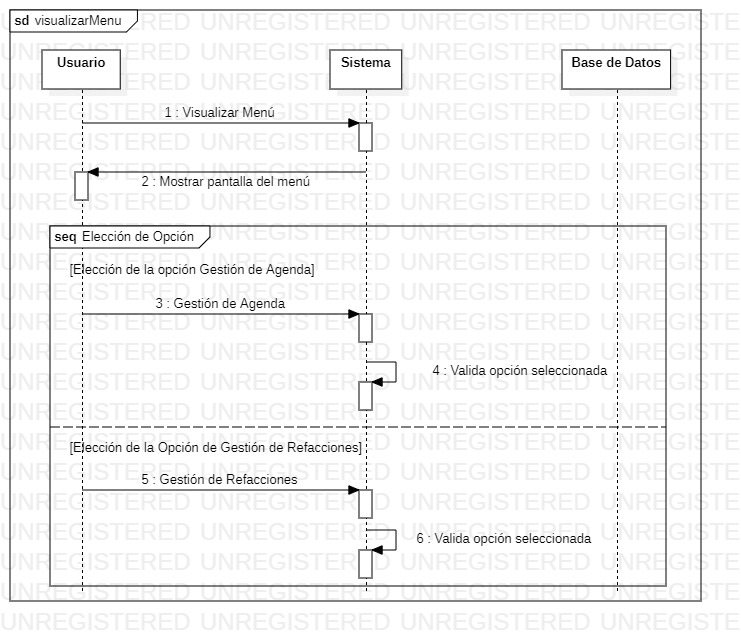
\includegraphics[width=0.9\textwidth]{./diseno/vprocesos/imagenes/visualizarMenu}
	\caption{Diagrama de Secuencia - Visualizar Menú}
	\label{fig:Diagrama de Secuencia - Visualizar Menú}
\end{figure}
%Documentación de los vehículos
\subsection{Visualizar Agenda}
En la siguiente figura \ref{fig:Diagrama de Secuencia - Visualizar Agenda} se muestra el diagrama de secuencia que corresponde a la visualización de la agenda que el Mecánico (Usuario) tiene en cuanto a los vehículos que va a reparar dentro del taller. Existen dos posibilidades dentro de esta actividad:
\begin{itemize}
	\item \textbf{Si existen registros:} Al momento de que el usuario entra a esta parte del sistema, al existir registros de vehículos por reparar, se muestra toda la información en una tabla y/o lista para su posterior gestión.  
	\item \textbf{No existen registros:} No hay vehículos registrados por reparar, se muestra una tabla y/o lista vacía en pantalla.
\end{itemize}
\begin{figure}[!h]
	\centering
	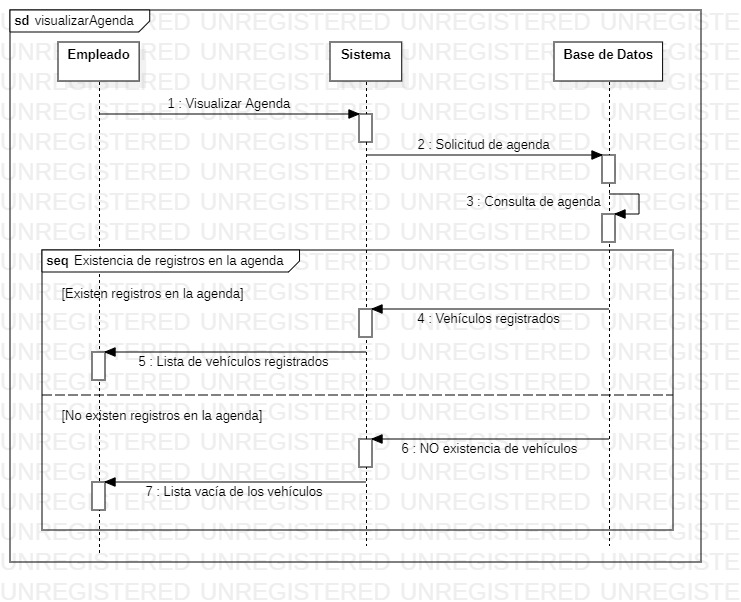
\includegraphics[width=1\textwidth]{./diseno/vprocesos/imagenes/visualizarAgenda}
	\caption{Diagrama de Secuencia - Visualizar Agenda}
	\label{fig:Diagrama de Secuencia - Visualizar Agenda}
\end{figure}
\subsubsection{Registrar Entrada de Vehículo}
En la figura \ref{fig:Diagrama de Secuencia - Registrar Entrada de Vehículo} se plasma el diagrama de secuencia que corresponde al registro de entrada de un vehículo al taller. El Mecánico (usuario) solicitará esta opción al sistema y este mismo le solicitará por medio de un formulario los datos necesarios para hacer el registro en la base de datos. Hay dos variantes en cuanto a la información ingresada: 
\begin{itemize}
	\item \textbf{Información válida:} Los datos que ha ingresado el usuario son válidos, es decir, que todos los campos han sido llenados y el formato del campo ingresado es el correcto. 
	\item \textbf{Información no válida:} Los datos que ha ingresado el usuario no son correctos. 
\end{itemize}
\begin{figure}[!h]
	\centering
	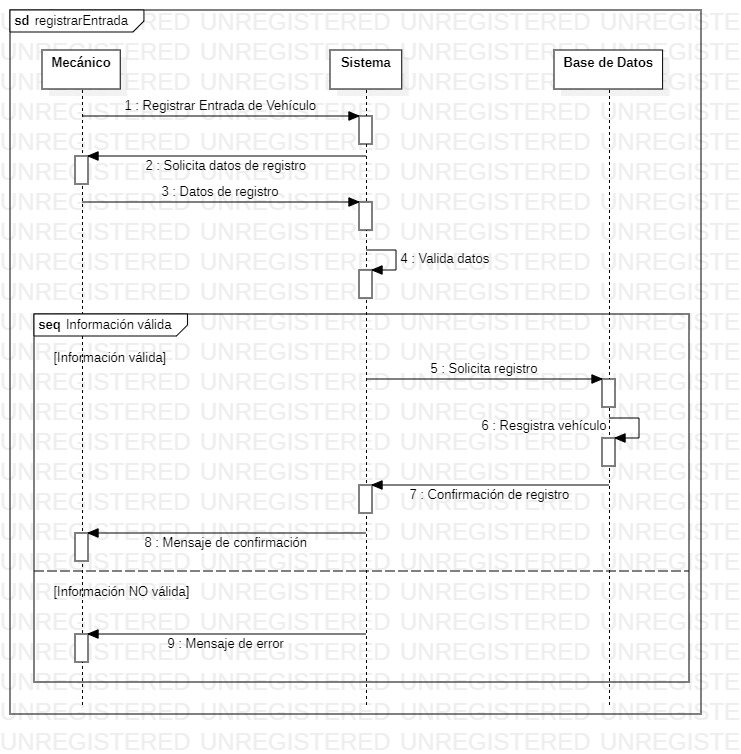
\includegraphics[width=0.8\textwidth]{./diseno/vprocesos/imagenes/registrarEntrada}
	\caption{Diagrama de Secuencia - Registrar Entrada de Vehículo}
	\label{fig:Diagrama de Secuencia - Registrar Entrada de Vehículo}
\end{figure}
\subsection{Modificar Entrada de Vehículo}
En la figura \ref{fig:Diagrama de Secuencia - Modificar Entrada de Vehículo} que se muestra a continuación se muestra el flujo de las diversas actividades que corresponden a la modificación de los datos de un registro de un vehículo. En este proceso, el usuario solicita esta modificación a través del sistema y este mismo interactúa con la base de datos para su modificación. En este proceso existen algunas variantes:
\begin{itemize}
	\item \textbf{Existe de vehículo:} Se corrobora que el vehículo está registrado en la base de datos, si es así, se procede a la modificación del mismo mediante un formulario de actualización.
	\item \textbf{No existe el vehículo:} Si no existe el vehículo en la base de datos, el sistema muestra un mensaje de error al usuario.
	\item \textbf{Datos válidos:} Al modificar los datos de un vehículo, el sistema valida si esa información es correcta, es decir, si los campos han sido llenados y el formato es el correspondiente con cada uno de dichos campos.
	\item \textbf{Datos no válidos:} Los datos que se quieren sobrescribir en la base de datos son incorrectos y el sistema no permite la actualización y muestra un mensaje de error.
\end{itemize}
\begin{figure}[!h]
	\centering
	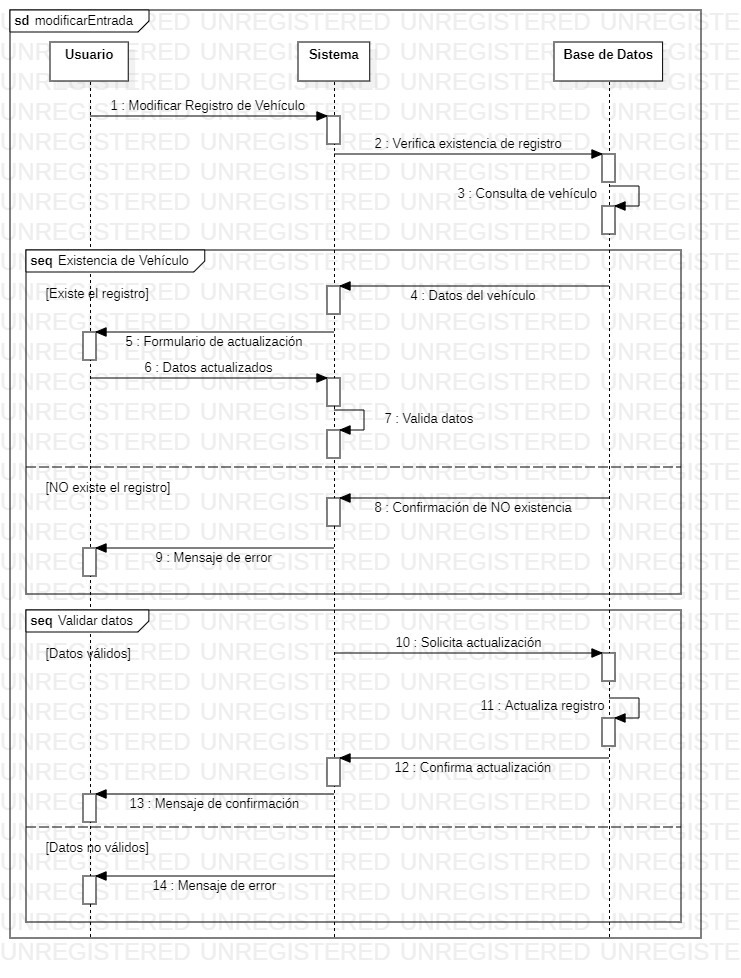
\includegraphics[width=1\textwidth]{./diseno/vprocesos/imagenes/modificarEntrada}
	\caption{Diagrama de Secuencia - Modificar Entrada de Vehículo}
	\label{fig:Diagrama de Secuencia - Modificar Entrada de Vehículo}
\end{figure}
\clearpage
\subsection{Eliminar Registro de Vehículo}
En la siguiente imagen \ref{fig:Diagrama de Secuencia - Eliminar Entrada de Vehículo}, se muestra el diagrama de secuencia correspondiente a la eliminación de algún registro para darle 'salida' al vehículo que se ha reparado. El sistema muestra un 'mensaje de seguridad' para verificar al usuario si esta seguro de borrar ese registro de la base de datos. Es en este punto donde el sistema toma dos caminos:
\begin{itemize}
	\item \textbf{Aceptación:} El Mecánico (usuario) acepta que desea eliminar ese registro, el sistema solicita a la base de datos la eliminación de dicho registro.
	\item \textbf{Cancelación:} Se elige la opción 'Cancelar' en la interfaz de usuario, el sistema desaparece el 'mensaje de seguridad' y la base de datos queda intacta. 
\end{itemize}
\begin{figure}[!h]
	\centering
	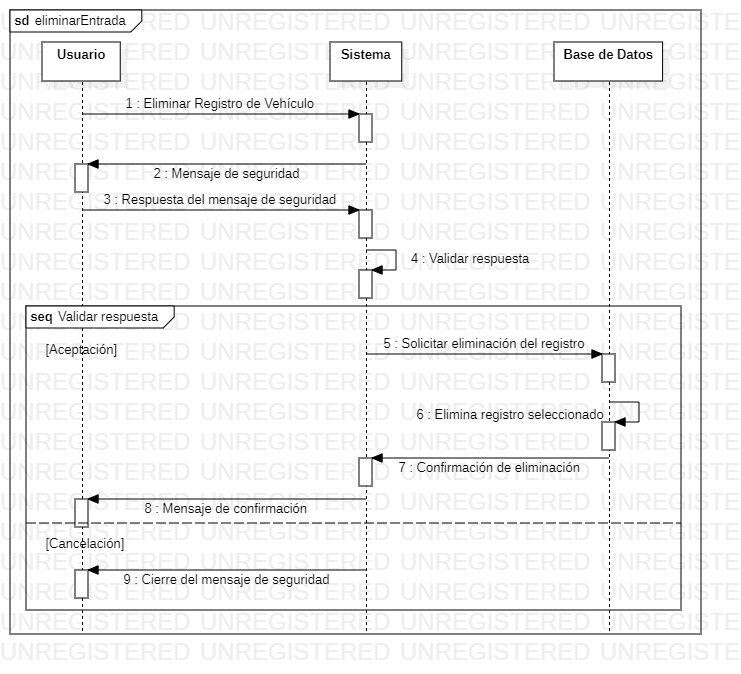
\includegraphics[width=0.9\textwidth]{./diseno/vprocesos/imagenes/eliminarEntrada}
	\caption{Diagrama de Secuencia - Eliminar Entrada de Vehículo}
	\label{fig:Diagrama de Secuencia - Eliminar Entrada de Vehículo}
\end{figure}
\clearpage
\subsection{Buscar Registro de Vehículo}
En la siguiente figura, la \ref{fig:Diagrama de Secuencia - Eliminar Entrada de Vehículo}, corresponde al diagrama de secuencia a la actividad de buscar algún registro de vehículo en específico, esto para ahorrar un poco más de tiempo en la búsqueda de ducho registro. Existen dos variantes en este proceso:
\begin{itemize}
	\item \textbf{Existe el registro:} Al encontrar el registro en la base de datos, se muestra en pantalla y se podrá interactuar con estos datos.
	\item \textbf{No existe el registro:} Si no se encuentra el registro, se mostrará en pantalla una lista y/o tabla en pantalla.
\end{itemize}
\begin{figure}[!h]
	\centering
	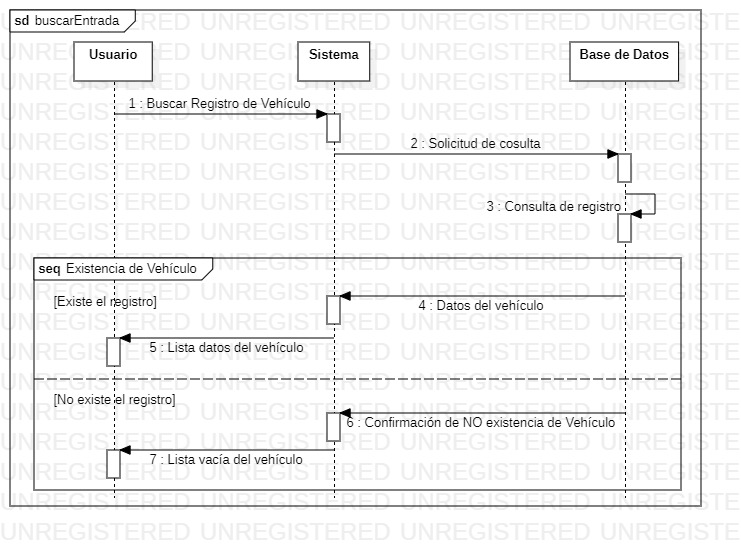
\includegraphics[width=1\textwidth]{./diseno/vprocesos/imagenes/buscarEntrada}
	\caption{Diagrama de Secuencia - Buscar Entrada de Vehículo}
	\label{fig:Diagrama de Secuencia - Buscar Entrada de Vehículo}
\end{figure}
 \clearpage
\subsubsection{Visualizar Refacciones Disponibles}
En la figura \ref{fig:Diagrama de Secuencia - Visualizar Refacciones} se muestra el diagrama de proceso que corresponde a la visualización de las refacciones que se encuentran en el almacén del taller. La aplicación hace la consulta a la base de datos y es aquí donde el software puede tomar dos opciones: 
\begin{itemize}
	\item \textbf{Existen registros:} Hay refacciones en almacenes, y se puede seleccionar alguna de ellas para implementarla en la reparación de un vehículo registrado.
	\item \textbf{No existen registros:} La base de datos manda un mensaje para la aplicación, la cual le muestra al Mecánico (usuario) una lista y/o tabla vacía. 
\end{itemize} 
\begin{figure}[!h]
	\centering
	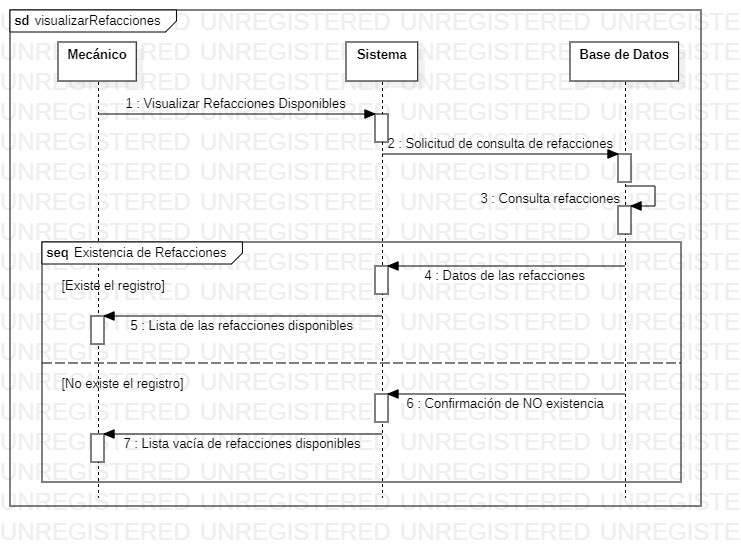
\includegraphics[width=1\textwidth]{./diseno/vprocesos/imagenes/visualizarRefacciones}
	\caption{Diagrama de Secuencia - Visualizar Refacciones}
	\label{fig:Diagrama de Secuencia - Visualizar Refacciones}
\end{figure}
\subsubsection{Solicitar Refacción}
En la siguiente figura \ref{fig:Diagrama de Secuencia - Solicitar Refaccion} se muestran la secuencia de las actividades que se deben de llevar a cabo para realizar la solicitud de una refacción que no se encuentre en el almacén del taller. El sistema solicita información al Mecánico (usuario) para generar una solicitud. Al ingresar datos al sistema, existe una validación de estos mismos datos, esto lleva al sistema a tomar dos caminos: 
\begin{itemize}
	\item \textbf{Información válida:} Los datos ingresados por el usuario son válidos, el formato y los campos han sido llenados correctamente de acuerdo a los datos que el sistema solicite.  
	\item \textbf{Información no válida:} Los datos ingresados por el usuario no son válidos, los campos o el formato no son correctos y el sistema muestra un mensaje de error.
\end{itemize} 
\begin{figure}[!h]
	\centering
	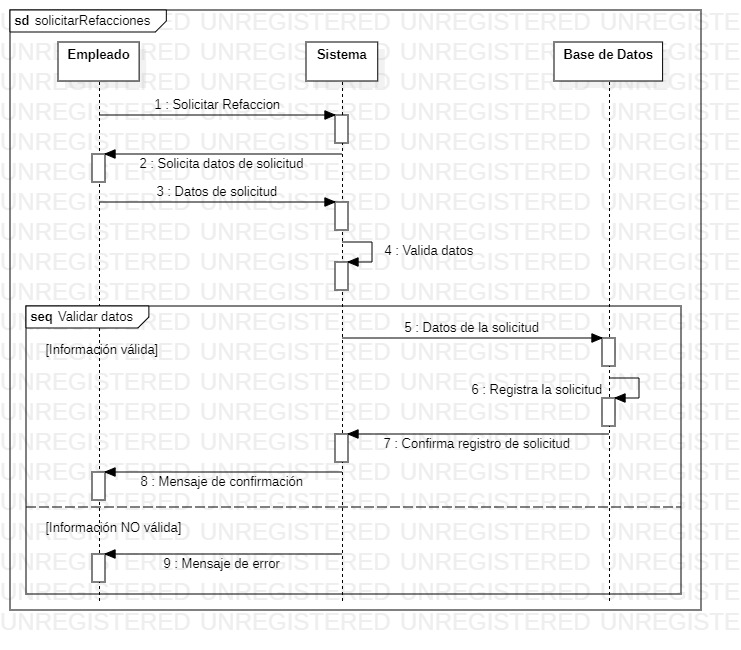
\includegraphics[width=0.9\textwidth]{./diseno/vprocesos/imagenes/solicitarRefacciones}
	\caption{Diagrama de Secuencia - Solicitar Refacción}
	\label{fig:Diagrama de Secuencia - Solicitar Refaccion}
\end{figure}
\clearpage
\subsection{Vista de Procesos Administrador}
El administrador también tiene poder sobre la gestión de los vehículos que entran al taller. Dicho poder lo comparte con el empleado, para visualizar mas a detalle estos procesos vea la sección de 'Vista de Procesos Empleado' \ref{subsec: Vista Procesos Empleado}.
%Documetnación de los empleados
\subsubsection{Visualizar Empleados}
En la siguiente figura \ref{fig:Diagrama de Secuencia - Visualizar Agenda} se muestra el diagrama de secuencia que corresponde a la visualización de cada uno de los registros de los empleados que existen dentro de la base de datos, existen dos posibilidades dentro de esta actividad:
\begin{itemize}
	\item \textbf{Si existen registros:} Al momento de que el administrador entra a esta parte del sistema, al existir registros de empleados, se muestra toda la información en una tabla y/o lista para su posterior gestión.  
	\item \textbf{No existen registros:} No hay empleados registrados, se muestra una tabla y/o lista vacía en pantalla.
\end{itemize}
\begin{figure}[!h]
	\centering
	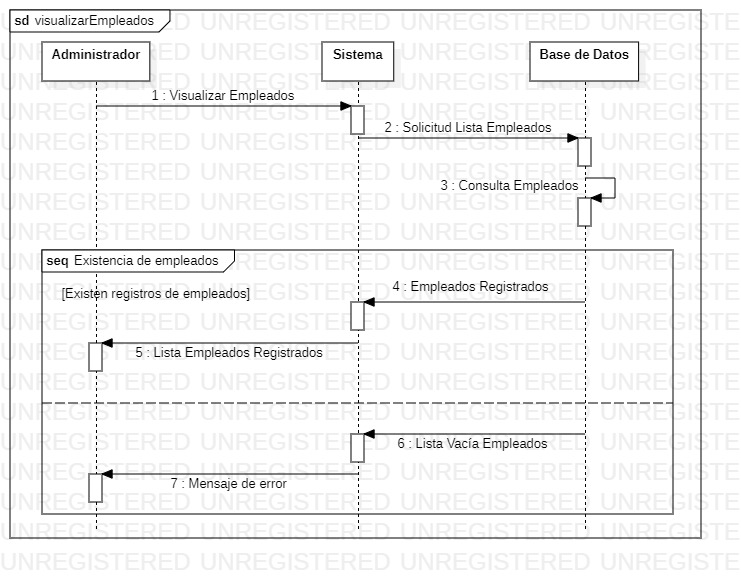
\includegraphics[width=0.8\textwidth]{./diseno/vprocesos/imagenes/visualizarEmpleados}
	\caption{Diagrama de Secuencia - Visualizar Empleados}
	\label{fig:Diagrama de Secuencia - Visualizar Empleados}
\end{figure}
\subsubsection{Registrar Nuevo Empleado}
En la figura \ref{fig:Diagrama de Secuencia - Registrar Nuevo Empleado} se plasma el diagrama de secuencia que corresponde al registro de un nuevo empleado dentro de la base de datos. El administrador solicitará esta opción al sistema y este mismo le solicitará por medio de un formulario los datos necesarios para hacer el registro en la base de datos. Hay dos variantes en cuanto a la información ingresada: 
\begin{itemize}
	\item \textbf{Información válida:} Los datos que ha ingresado el administrador son válidos, es decir, que todos los campos han sido llenados y el formato del campo ingresado es el correcto. 
	\item \textbf{Información no válida:} Los datos que ha ingresado el usuario no son correctos. 
\end{itemize}
\begin{figure}[!h]
	\centering
	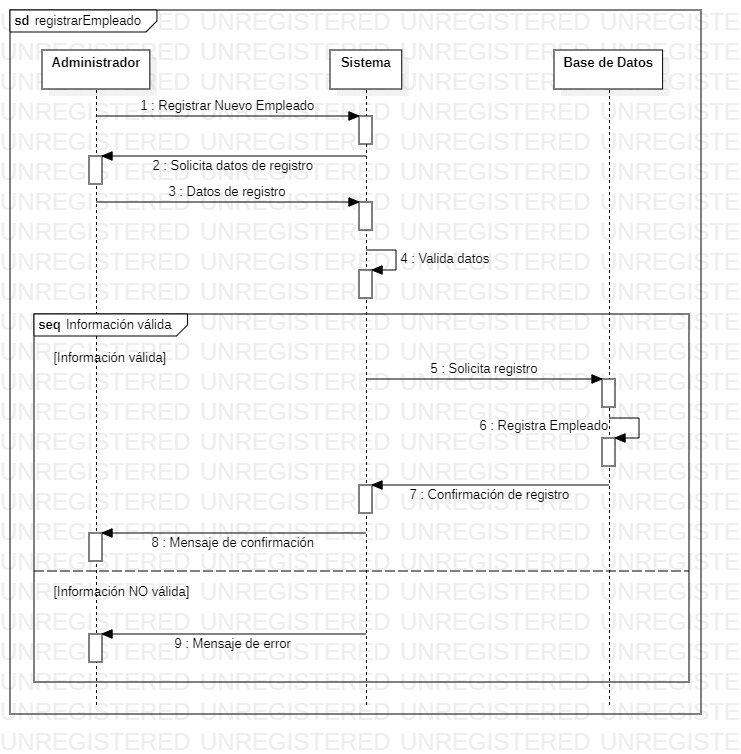
\includegraphics[width=0.8\textwidth]{./diseno/vprocesos/imagenes/registrarEmpleado}
	\caption{Diagrama de Secuencia - Registrar Nuevo Empleado}
	\label{fig:Diagrama de Secuencia - Registrar Nuevo Empleado}
\end{figure}
\subsubsection{Modificar Empleado}
En la figura \ref{fig:Diagrama de Secuencia - Modificar Empleado} que se muestra a continuación se muestra el flujo de las diversas actividades que corresponden a la modificación de los datos de un registro de un empleado. En este proceso, el administrador solicita esta modificación a través del sistema y este mismo interactúa con la base de datos para su modificación. En este proceso existen algunas variantes:
\begin{itemize}
	\item \textbf{Existe empleado:} Se asegura que el empleado está registrado en la base de datos, si es así, se procede a la modificación del mismo mediante un formulario de actualización.
	\item \textbf{No existe el empleado:} Si no existe el registro del empleado en la base de datos, el sistema muestra un mensaje de error al usuario.
	\item \textbf{Datos válidos:} Al modificar los datos de un empleado, el sistema valida si esa información es correcta, es decir, si los campos han sido llenados y el formato es el correspondiente con cada uno de dichos campos.
	\item \textbf{Datos no válidos:} Los datos que se quieren sobrescribir en la base de datos son incorrectos y el sistema no permite la actualización y muestra un mensaje de error.
\end{itemize}
\begin{figure}[!h]
	\centering
	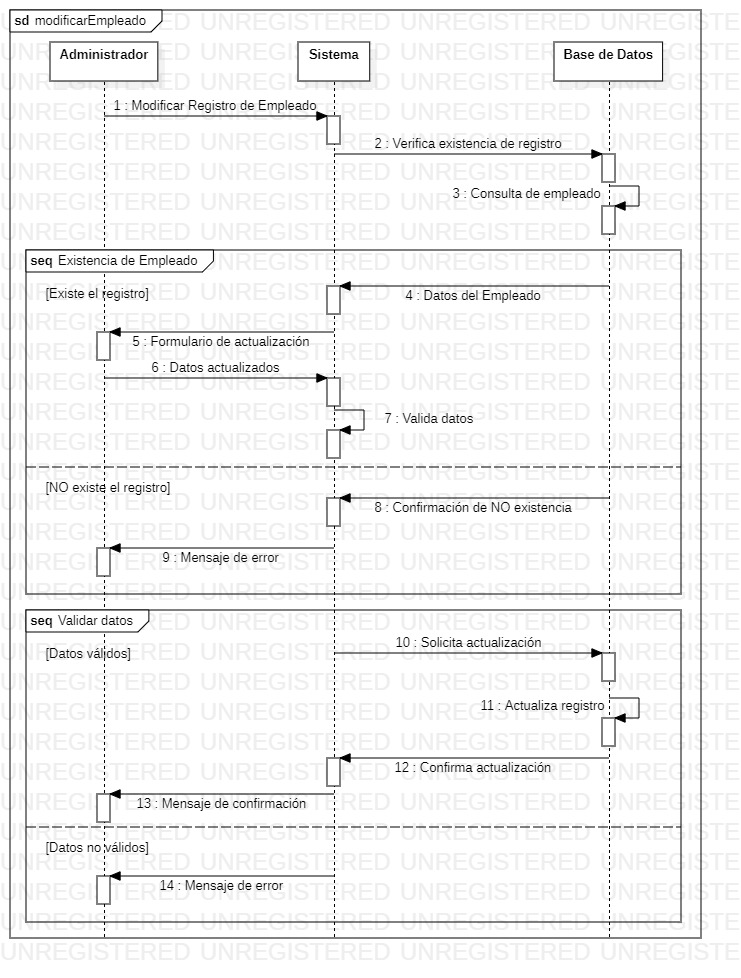
\includegraphics[width=1\textwidth]{./diseno/vprocesos/imagenes/modificarEmpleado}
	\caption{Diagrama de Secuencia - Modificar Empleado}
	\label{fig:Diagrama de Secuencia - Modificar Empleado}
\end{figure}
\clearpage
\subsubsection{Eliminar Empleado}
En la siguiente imagen \ref{fig:Diagrama de Secuencia - Eliminar Empleado}, se muestra el diagrama de secuencia correspondiente a la eliminación de algún registro de un empleado, esto en el caso de que ya no pertenezca a la organización o simplemente renunció. El sistema muestra un 'mensaje de seguridad' para verificar al administrador si esta seguro de borrar ese registro de la base de datos. Existen dos posibilidades dentro de este módulo:
\begin{itemize}
	\item \textbf{Aceptación:} El administrador acepta que desea eliminar ese registro, el sistema solicita a la base de datos la eliminación de dicho registro y se muestra un mensaje de que el empleado ha sido eliminado de manera satisfactoria.
	\item \textbf{Cancelación:} Si elige la opción 'Cancelar' en la interfaz de usuario, el sistema desaparece el 'mensaje de seguridad' y la base de datos queda intacta. 
\end{itemize}
\begin{figure}[!h]
	\centering
	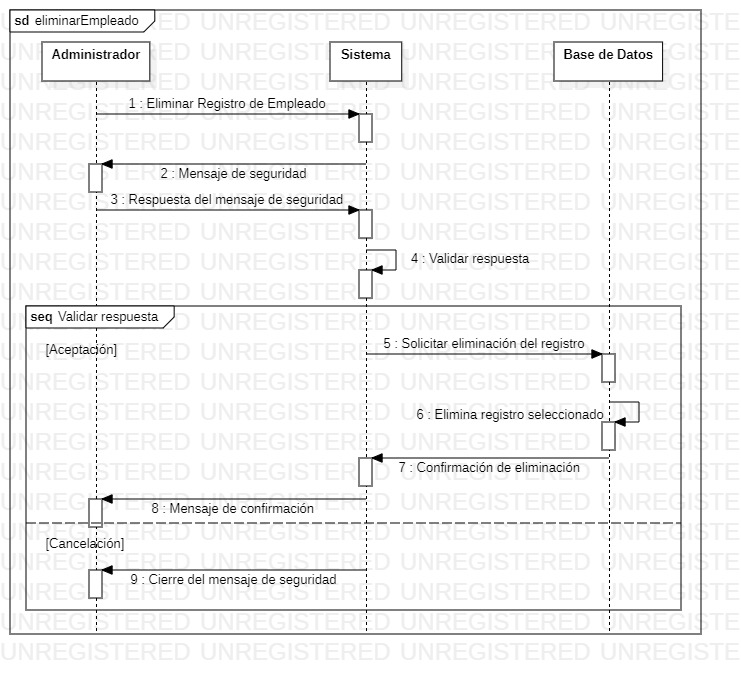
\includegraphics[width=0.8\textwidth]{./diseno/vprocesos/imagenes/eliminarEmpleado}
	\caption{Diagrama de Secuencia - Eliminar Empleado}
	\label{fig:Diagrama de Secuencia - Eliminar Empleado}
\end{figure}
\clearpage
\subsubsection{Buscar Registro de Vehículo}
En el siguiente diagrama, la \ref{fig:Diagrama de Secuencia - Eliminar Entrada de Vehículo}, corresponde la secuencia de actividades para buscar algún registro de un empleado en específico, esto para ahorrar un poco más de tiempo en la búsqueda de ducho registro y poder realizar alguna acción sobre ese registro. Existen dos variantes en este proceso:
\begin{itemize}
	\item \textbf{Existe el registro:} Al encontrar el registro en la base de datos, se muestra en pantalla y se podrá interactuar con estos datos.
	\item \textbf{No existe el registro:} Si no se encuentra el registro, se mostrará en pantalla una lista y/o tabla en pantalla.
\end{itemize}
\begin{figure}[!h]
	\centering
	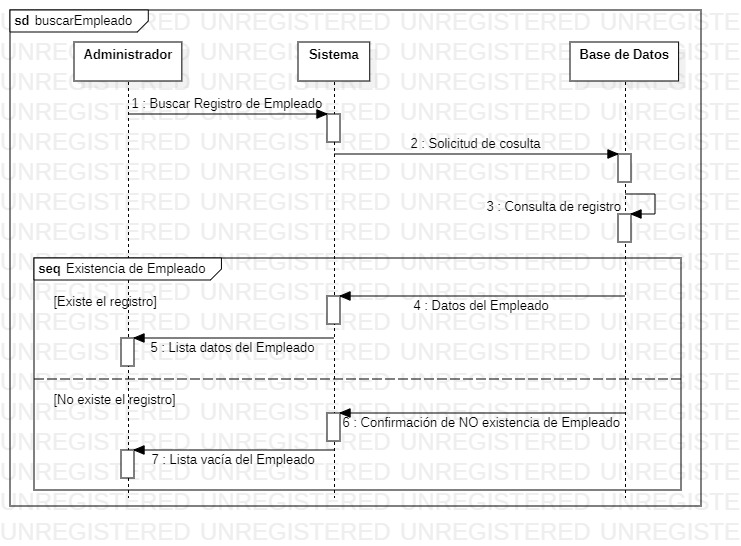
\includegraphics[width=1\textwidth]{./diseno/vprocesos/imagenes/buscarEmpleado}
	\caption{Diagrama de Secuencia - Buscar Empleado}
	\label{fig:Diagrama de Secuencia - Buscar Empleado}
\end{figure}
\clearpage
%Documentación de las refacciones
\subsubsection{Registrar Refacción}
En la siguiente figura \ref{fig:Diagrama de Secuencia - Registrar Refaccion} se muestra el diagrama de secuencia que corresponde al registro de una refacción que vaya a entrar al almacén, esta puede haber sido solicitada por un empleado o no. El administrador solicitará esta opción al sistema y este mismo le solicitará por medio de un formulario los datos necesarios para hacer el registro en la base de datos. Hay dos variantes en cuanto a la información ingresada: 
\begin{itemize}
	\item \textbf{Información válida:} Los datos que ha ingresado el administrador son válidos, es decir, que todos los campos han sido llenados y el formato del campo ingresado es el correcto. 
	\item \textbf{Información no válida:} Los datos que ha ingresado el usuario no son correctos. 
\end{itemize}
\begin{figure}[!h]
	\centering
	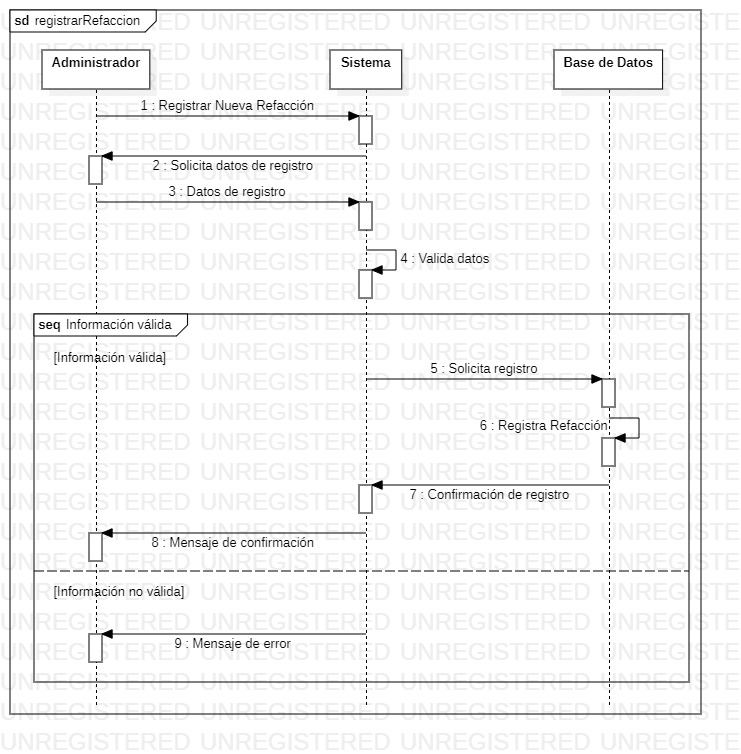
\includegraphics[width=0.8\textwidth]{./diseno/vprocesos/imagenes/registrarRefaccion}
	\caption{Diagrama de Secuencia - Registrar Refacción}
	\label{fig:Diagrama de Secuencia - Registrar Refaccion}
\end{figure}
\subsubsection{Modificar Refacción}
En la figura \ref{fig:Diagrama de Secuencia - Modificar Empleado} se muestra el flujo de las diversas actividades que corresponden a la modificación de los datos de una refacción que se encuentra en almacén del taller, esto en dado caso que haya un error en la captura de dichos datos. En este proceso, el administrador solicita esta modificación a través del sistema y este mismo interactúa con la base de datos para su modificación. En este proceso existen tres variantes para los datos a modificar:
\begin{itemize}
	\item \textbf{Existe empleado:} Se asegura que la refacción está registrada,en dado caso que si, se procede a la modificación del mismo mediante un formulario de actualización.
	\item \textbf{No existe el empleado:} Si no existe el registro de la refacción en la base de datos, el sistema muestra un mensaje de error al usuario.
	\item \textbf{Datos válidos:} Al modificar los datos de un empleado, el sistema valida si esa información es correcta, es decir, si los campos han sido llenados y el formato es el correspondiente con cada uno de dichos campos.
	\item \textbf{Datos no válidos:} Los datos que se quieren sobrescribir en la base de datos son incorrectos y el sistema no permite la actualización y muestra un mensaje de error.
\end{itemize}
\begin{figure}[!h]
	\centering
	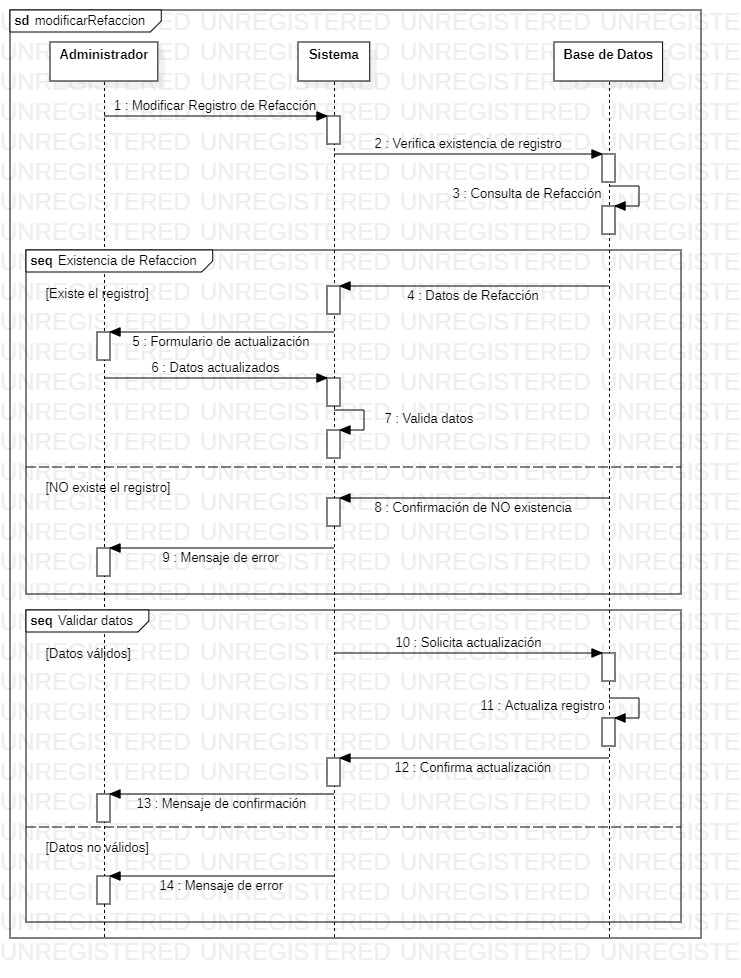
\includegraphics[width=1\textwidth]{./diseno/vprocesos/imagenes/modificarRefaccion}
	\caption{Diagrama de Secuencia - Modificar Refacción}
	\label{fig:Diagrama de Secuencia - Modificar Refaccion}
\end{figure}
\clearpage
\subsubsection{Eliminar Refaccion}
En la siguiente imagen \ref{fig:Diagrama de Secuencia - Eliminar Refaccion}, se muestra el diagrama de secuencia correspondiente a la eliminación de algún registro de una refacción que estaba en alamcén del taller, esto en el caso de que ya no haya en existencia o el proveedor no las haya conseguido. El sistema muestra un 'mensaje de seguridad' para verificar al administrador si esta seguro de borrar ese registro de la base de datos. Existen dos posibilidades dentro de este módulo:
\begin{itemize}
	\item \textbf{Aceptación:} El administrador acepta que desea eliminar ese registro, el sistema solicita a la base de datos la eliminación de dicho registro y se muestra un mensaje de que el empleado ha sido eliminado de manera satisfactoria.
	\item \textbf{Cancelación:} Si elige la opción 'Cancelar' en la interfaz de usuario, el sistema desaparece el 'mensaje de seguridad' y la base de datos queda intacta. 
\end{itemize}
\begin{figure}[!h]
	\centering
	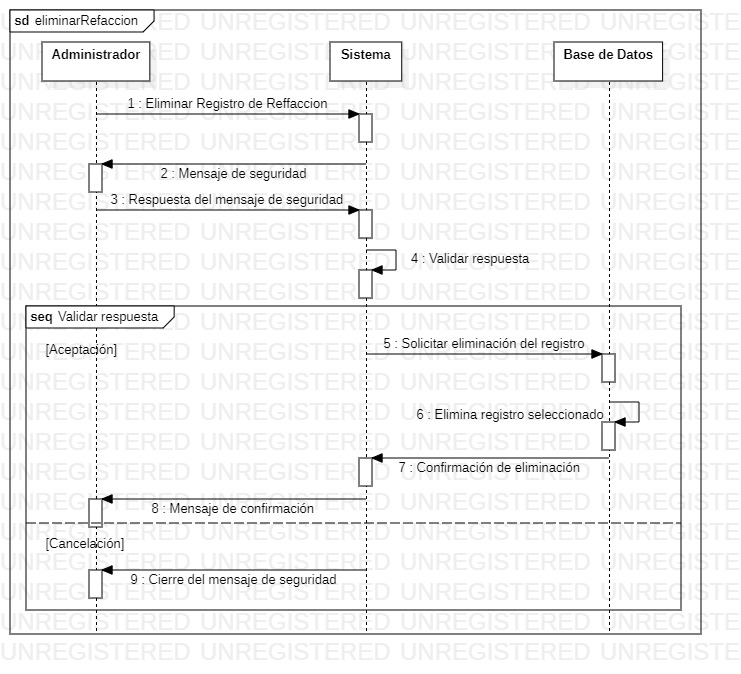
\includegraphics[width=0.8\textwidth]{./diseno/vprocesos/imagenes/eliminarRefaccion}
	\caption{Diagrama de Secuencia - Eliminar Refacción}
	\label{fig:Diagrama de Secuencia - Eliminar Refaccion}
\end{figure}
\clearpage
\subsubsection{Buscar Refacción}
En el siguiente diagrama, la \ref{fig:Diagrama de Secuencia - Eliminar Entrada de Vehículo}, corresponde la secuencia de actividades para buscar algún registro de un empleado en específico, esto para ahorrar un poco más de tiempo en la búsqueda de ducho registro y poder realizar alguna acción sobre ese registro. Existen dos variantes en este proceso:
\begin{itemize}
	\item \textbf{Existe el registro:} Al encontrar el registro en la base de datos, se muestra en pantalla y se podrá interactuar con estos datos.
	\item \textbf{No existe el registro:} Si no se encuentra el registro, se mostrará en pantalla una lista y/o tabla en pantalla.
\end{itemize}
\begin{figure}[!h]
	\centering
	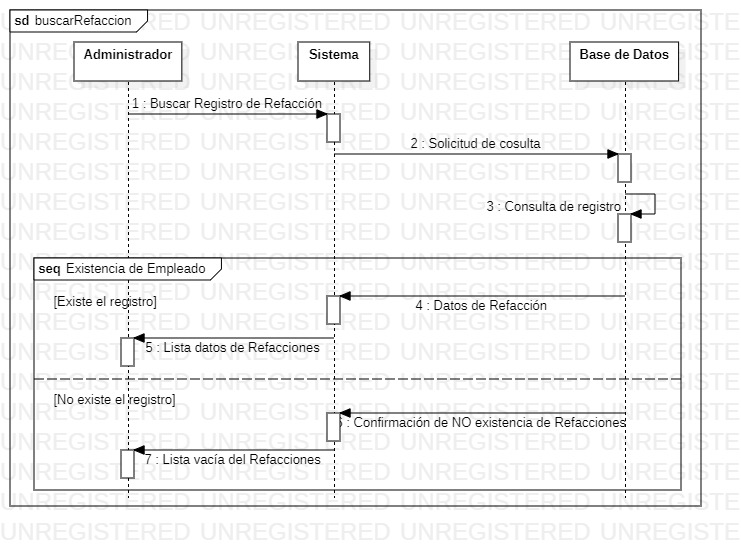
\includegraphics[width=1\textwidth]{./diseno/vprocesos/imagenes/buscarRefaccion}
	\caption{Diagrama de Secuencia - Buscar Refacción}
	\label{fig:Diagrama de Secuencia - Buscar Refaccion}
\end{figure}
\clearpage
%Documetnación de solicitudes
\subsubsection{Visualizar Solicitud}
En la siguiente figura \ref{fig:Diagrama de Secuencia - Visualizar Solicitudes de Refaccion} se muestra el diagrama de secuencia que corresponde a la visualización de todas las solicitudes que los diversos empleados han realizado para que puedan hacer su trabajo, existen dos posibilidades dentro de esta actividad:
\begin{itemize}
	\item \textbf{Si existen registros:} Al momento de que el administrador entra a esta parte del sistema, se muestra en una tabla y/o lista toda la información necesaria para atender a las solicitudes que se necesiten.  
	\item \textbf{No existen registros:} No hay empleados registrados, se muestra una tabla y/o lista vacía en pantalla.
\end{itemize}
\begin{figure}[!h]
	\centering
	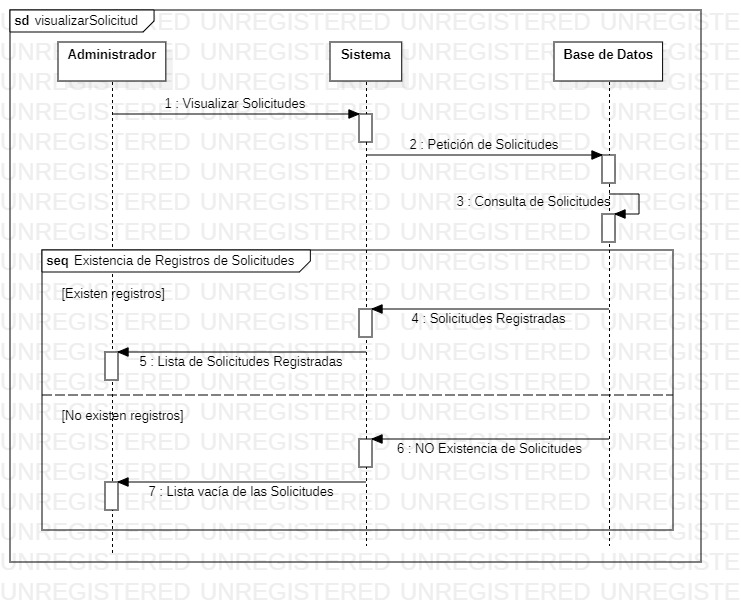
\includegraphics[width=0.8\textwidth]{./diseno/vprocesos/imagenes/visualizarSolicitud}
	\caption{Diagrama de Secuencia - Visualizar Solicitudes de Refacción}
	\label{fig:Diagrama de Secuencia - Visualizar Solicitudes de Refaccion}
\end{figure}
\clearpage
\subsubsection{Atender Solicitud}
En en siguiente diagrama\ref{fig:Diagrama de Secuencia - Visualizar Solicitudes de Refaccion} se muestra la secuencia que corresponde a la atención de todas las solicitudes que los diversos empleados han realizado para que puedan hacer su trabajo, al momento de aceptar la solicitud y atenderla el administrador ingresará unos datos que el sistema solicite, estos datos tendrán que ser verificados:
\begin{itemize}
	\item \textbf{Datos válidos:} Los datos ingresados por el administrador son correctos y cuentan con el formato específico para ser ingresados a la base de datos y atender a la solicitud del empleado.  
	\item \textbf{Datos no válidos} Los datos ingresados no son correctos o no cumplen con las especificaciones de formato.
\end{itemize}
\begin{figure}[!h]
	\centering
	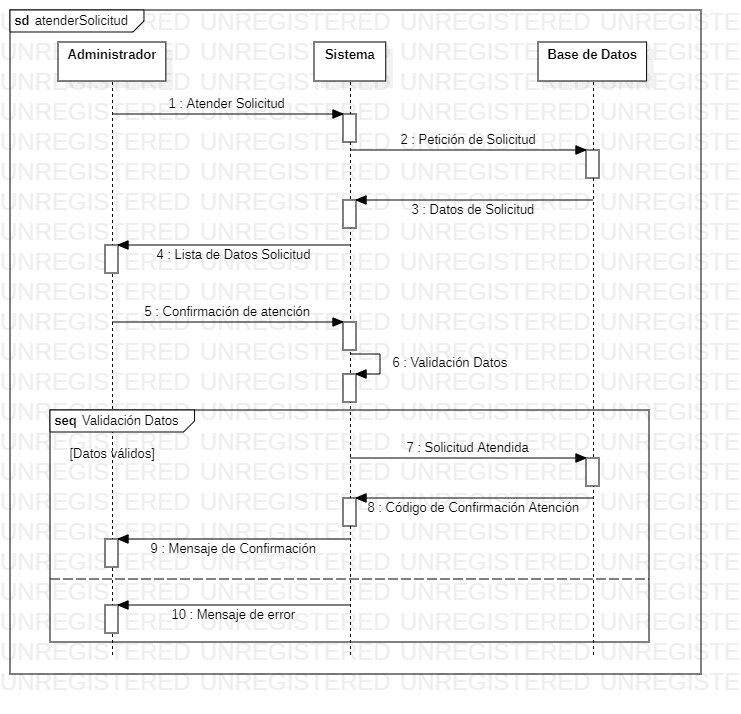
\includegraphics[width=0.8\textwidth]{./diseno/vprocesos/imagenes/atenderSolicitud}
	\caption{Diagrama de Secuencia - Atender Solicitud de Refacción}
	\label{fig:Diagrama de Secuencia - Atender Solicitud de Refaccion}
\end{figure}
\clearpage

